\chapter{Machine Learning}%
\label{ch:ml}

The next chapter is somewhat of a diversion from the physics discussed so far.
It will focus on techniques in machine learning which are often referred to in
High Energy Physics as a Multi-variate Analysis (MVA). The reason for this
diversion is that these techniques have become very widespread in the field,
they are used in several of the reconstruction and selection algorithms that are
used to obtain the events on which the analysis is performed. Furthermore an MVA
is used to obtain the distribution that acts as the final discriminant for the
analysis, and machine learning techniques are also used to model the
backgrounds. Given how widespread the use of these techniques is in the analysis
it makes sense to describe them before diving into the details.

The two main algorithms used are Boosted Decision Trees (BDTs) and Neural
Networks (NNs) which will be described in sections~\ref{sec:bdts}
and~\ref{sec:neural-networks} respectively. These algorithms are used in many
places outside High Energy Physics and so rather than referring to individual
pieces of data that enter into the algorithm as an event, in this chapter they
will be referred to as an example. This terminology comes from the fact that in
general these algorithms must be shown a large number of examples before they
are suitable ``trained'' for their purpose, and that in general those examples
could be data that represent anything. Both of these algorithms can be operated
in classification or regression modes. The main difference between these modes
is that classification mode provides a score for each of a given number of
classes which can be interpreted as a probability that a given example belongs
to the given class, whereas regression outputs a single number per example whose
interpretation depends on the problem.

Both algorithms can be written as a function of some inputs $\vec{x}$, some
weights to be found during training $\vec{w}$, and a set of hyper-parameters
$\vec{\theta}$ as follows
\begin{equation}
  F(\vec{x}, \vec{w}, \vecv{\theta}) = \vec{y},
\end{equation}
where $\vec{y}$ is a vector whose outputs correspond to each class in a
classification problem. If the algorithm is set up for a regression problem then
the output will just be one number. Training either algorithm involves an
iterative process where at each iteration the function is evaluated for the
current set of weights, the outputs are compared against some truth labels
$\vec{t}$ via the computation of a loss function. Based on the value of the loss
function the weights are then updated according to the given algorithm. It is
therefore vital that firstly these truth labels are available for the data on
which one wants to train (e.g. train on simulated predictions rather than real
data) and secondly that the examples are split into a training and testing set
so that the set which is used to iteratively update weights is not the same set
that performance is evaluated on. This avoids over-fitting to any noise in a
given set, though this problem is not circumvented entirely and over-fitting
will be addressed for specific algorithms in the sections ahead.

\section{Boosted Decision Trees}%
\label{sec:bdts}
We will start by discussing a decision tree for a classification problem.
Decision trees have a structure as in figure~\ref{fig:bdt}, which shows a tree
dividing examples into two classes, red and blue.
\begin{figure}[h]
  \centering
  \begin{tikzpicture}
    \draw [very thick] plot [smooth] coordinates {(-5,-3) (5,3)};
    \draw [very thick] plot [smooth] coordinates {(-5, 3) (5,-3)};
  \end{tikzpicture}
  \caption{The structure of a decision tree.}
  \label{fig:bdt}
\end{figure}


Each circular node in the tree represents a cut on one of a number of variables
provided as input to the algorithm. The tree is read top to bottom with each
node being followed by two edges branching left and right that represent the
path taken by examples which pass or fail the cut respectively. Square nodes
represent that the termination criteria have been reached and that events in
these nodes have been classified according to the colour of the node. The
variable chosen at each node is optimised in order to maximise a criteria
related to the separation of classes.  For a problem containing two classes a
common separation criteria is the Gini index,
\begin{equation}
  G = p(1-p),
  \label{eq:gini}
\end{equation}
where p is the purity of a chosen class that one wants to maximise.

A decision tree by itself is able to separate examples into a number of classes,
however a single tree is prone to over--training. Over--training is the term
used to describe the phenomena where a classifier learns from statistical
fluctuations in the data rather learning a generalised separation boundary
between classes. The reason that decision trees are susceptible to this is that
if two variables yield a similar separation criteria then a fluctuation in the
training data may lead to the choice of one variable over another for a
particular node, this choice will lead to a very different tree structure than
if the fluctuation were not present.

In order to mitigate the over--training tendencies of decision trees they are
often used in an ensemble algorithm such as bagging~\cite{bagging}
or boosting~\cite{boosting}. Here only boosting will be discussed. Ensembles of
decision trees are often referred to as random forests. Boosting works by
training a sequence of trees, weighting misclassified events from a tree so that
they have more influence over the structure of the next tree in the sequence.
The final classification of any given example is a weighted average over all
trees, this can be weighted by the overall accuracy of each tree, but in general
can take any weighted average.

\subsection{Gradient Boosting}

Gradient boosting is the name of an optimisation algorithm that takes the
concept of boosting and combines it with the gradient descent algorithm. A
pictographic representation of gradient descent for a regression problem can be
seen in figure~\ref{fig:grad-desc.}
\begin{figure}[ht]
  \centering
  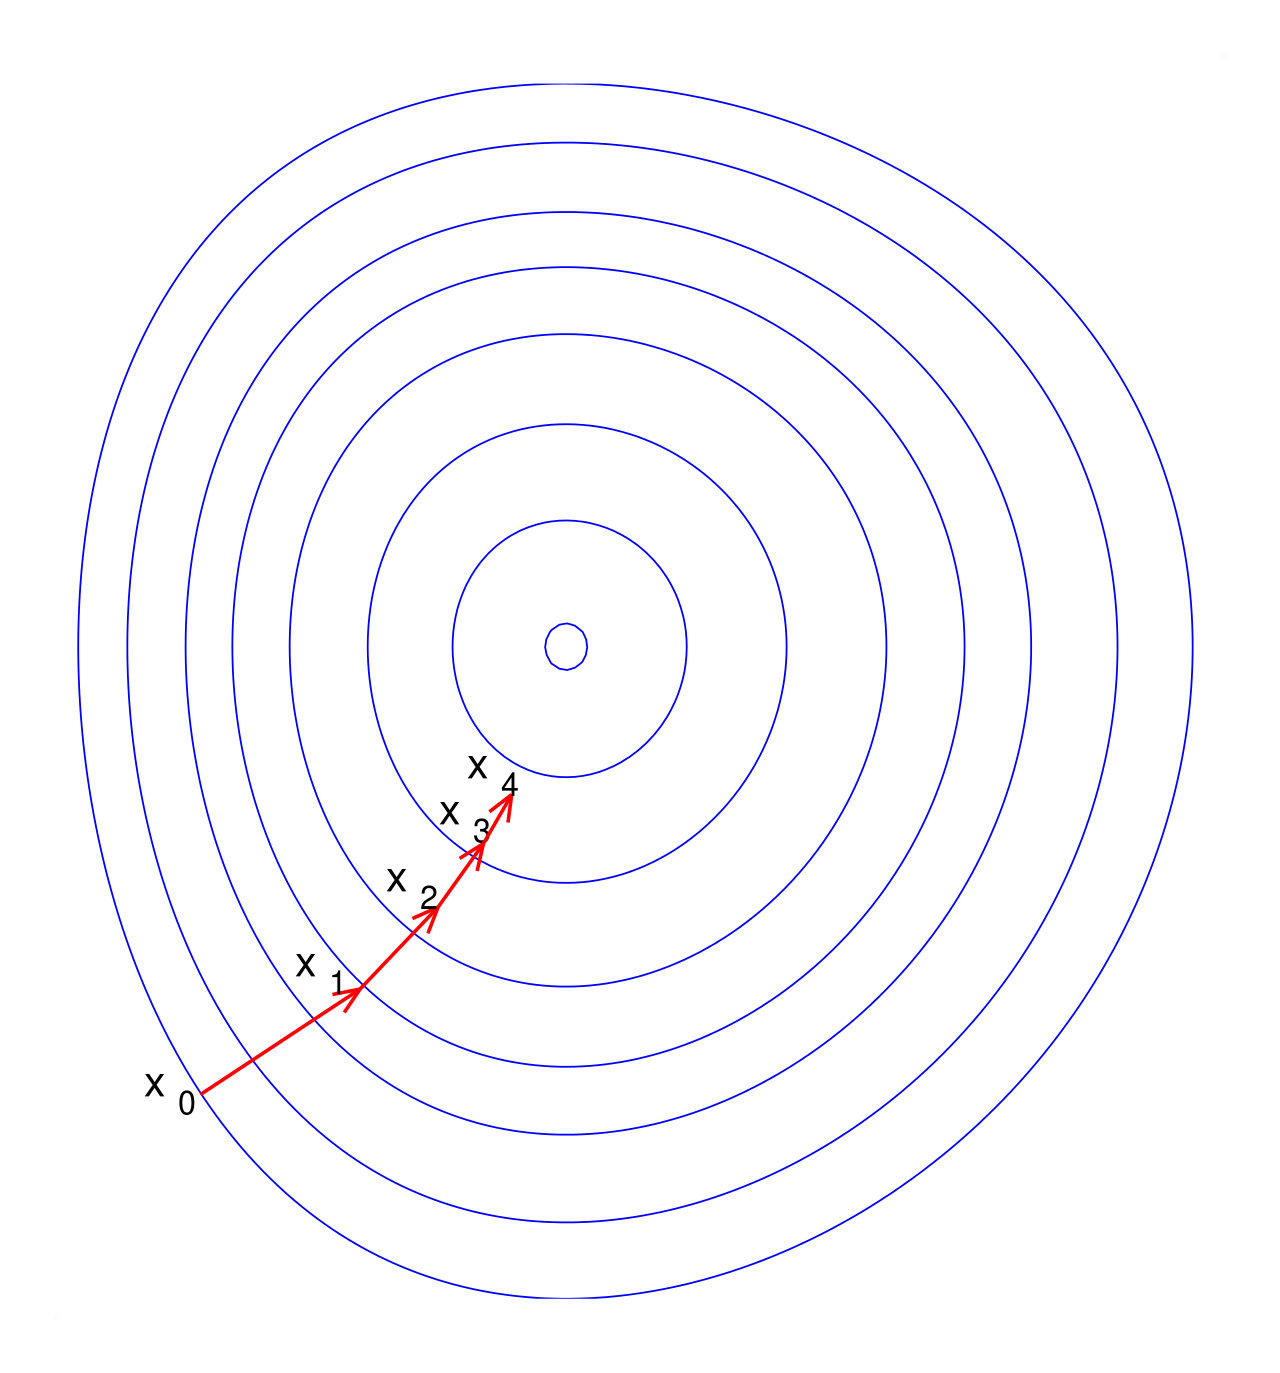
\includegraphics[width=.6\textwidth]{gradient-descent}
  \caption[An illustration of gradient descent.]{An illustration of the gradient
    descent algorithm. The blue lines represent level sets of a function, sets
    of points that have the same gradient. The $x$'s represent where in along
    the function the algorithm is at a given step with the steps numbered 0 to
    4.}
  \label{fig:grad-desc}
\end{figure}
  

\section{Neural Networks}%
\label{sec:neural-networks}
Neural networks have a structure as in figure~\ref{fig:nn}.

This section outlines some of the mathematical formalism surrounding NNs
that act as classifiers. These kinds of NNs can be used to solve binary
classification or multi-class problems, where the probability that each data
candidate belongs to any of the classes is mutually exclusive. Many other types
of NN exist, however their details will not be discussed in this work. In simple
terms a NN is comprised of connected layers of nodes as in figure
\ref{fig:basicnn}. Nodes fall into three types input, output and hidden, with
layers being homogeneous with regard to node type and therefore inheriting their
name. The input layer is comprised of one input node per dimension of a single
entry in the dataset that one wishes to pass into the NN for classification.
Each output node is a predictive unit corresponding to one of $K$ classes and it
is the goal of the intermediate hidden layers (full of hidden units) to provide
a relationship between the inputs and outputs such that the predictive unit with
the highest value corresponds to the correct class for the given data. The
output layer should therefore be comprised of $K$ nodes. In order to delve
further into the details, a good mathematical representation of the hidden
layers is required. One such representation is given by Bishop in Pattern
Recognition and Machine Learning \cite{PRML}. In this section the nomenclature
used by Bishop will be outlined and then adapted for our specific use.

\tikzset{%
  every neuron/.style={
    circle,
    minimum size=22pt,
    draw
  },
  neuron missing/.style={
    draw=none, 
    scale=3,
    text height=0.3cm,
    execute at end node=\color{black}\tiny{$\vdots$}
  },
}

\begin{figure}[hbtp]
  \centering
  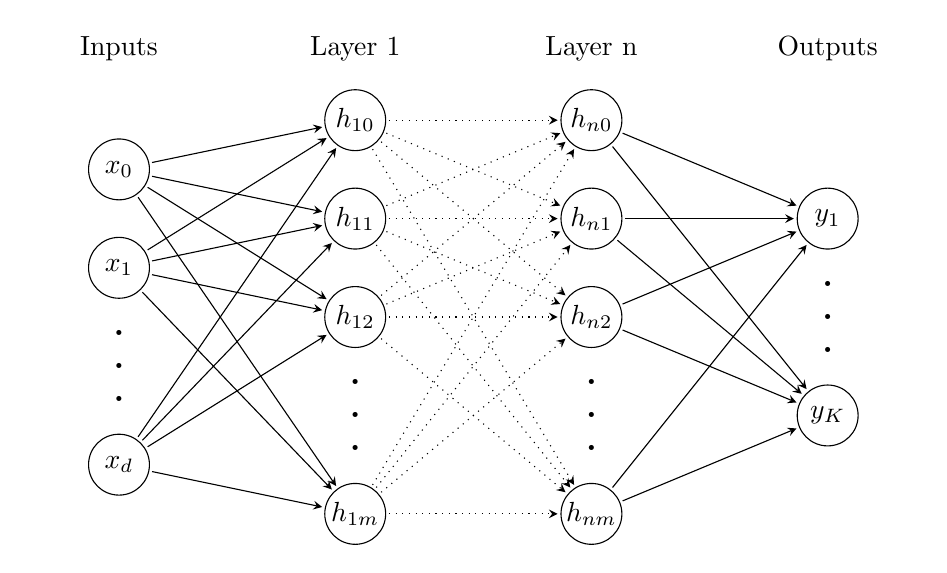
\begin{tikzpicture}[x=1.5cm, y=1.25cm, >=stealth]
    
    \foreach \m/\l [count=\y] in {1,2,missing,3}
    \node [every neuron/.try, neuron \m/.try] (input-\m) at (0,2-\y) {};

    \foreach \m [count=\y] in {1,2,3,missing,4}
    \node [every neuron/.try, neuron \m/.try ] (hidden1-\m) at (2,2.5-\y) {};

    \foreach \m [count=\y] in {1,2,3,missing,4}
    \node [every neuron/.try, neuron \m/.try ] (hidden2-\m) at (4,2.5-\y) {};

    \foreach \m [count=\y] in {1,missing,2}
    \node [every neuron/.try, neuron \m/.try ] (output-\m) at (6,1.5-\y) {};

    \foreach \l [count=\i] in {0,1,d}
    \node at (input-\i.center) {$x_{\l}$};

    \foreach \l [count=\i] in {0,1,2,m}
    \node at (hidden1-\i.center) {$h_{1\l}$};

    \foreach \l [count=\i] in {0,1,2,m}
    \node at (hidden2-\i.center) {$h_{n\l}$};

    \foreach \l [count=\i] in {1,K}
    \node at (output-\i.center) {$y_\l$};

    \foreach \i in {1,...,3}
    \foreach \j in {1,...,4}
    \draw [->, shorten <=1pt, shorten >=1pt] (input-\i) -- (hidden1-\j);

    \foreach \i in {1,...,4}
    \foreach \j in {1,...,4}
    \draw [dotted, ->, shorten <=1pt, shorten >=1pt] (hidden1-\i) -- (hidden2-\j);

    \foreach \i in {1,...,4}
    \foreach \j in {1,...,2}
    \draw [->, shorten <=1pt, shorten >=1pt] (hidden2-\i) -- (output-\j);

    \foreach \l [count=\x from 0] in {Inputs, Layer 1, Layer n, Outputs}
    \node [align=center, above] at (\x*2,2) {\l};
  \end{tikzpicture}
  \caption[A depiction of a neural network.]{A more complex neural network
    containing an input layer of $d$ nodes corresponding to data of dimensionality
    $d$, $n$ hidden layers of $m$ hidden units each $h_{ij}$ (where $i$ indexes
    hidden layer and $j$ indexes a particular unit) and an output layer of $K$
    predictive units $y_k$.}
  \label{fig:nn}
\end{figure}
The building blocks of the NN, called activations, resemble Fisher
discriminants \cite{Fisher} and take the form

\begin{equation}
a_j = \sum_{i=1}^{d} w_{ji}x_{i} + w_{j0}
\label{eq:fisher}
\end{equation}
where the $w_{ji}$ terms are known as weights and the $w_{j0}$ as biases.
Collectively the weights and biases shall be referred to as adaptive parameters,
due to the fact that (as shall be made clear later) they are to be adapted by a
training algorithm. In order to take the activations and turn them into
something closer to a perceptron \cite{Rosenblatt} they must be passed through
an activation function denoted $\mathcal{H}$,

\begin{equation}
h_j = \mathcal{H}(a_j)
\label{eq:hiddenunit}
\end{equation}
becoming what are known as hidden units. These activation functions may be
non-linear and have the restriction that they must be differentiable, crucially
this is different from the perceptron which uses a non-differentiable step
function. Considering a network with only a single hidden layer as in figure
\ref{fig:basicnn}, there are further steps required to get from the hidden units
to the predictions $y_k$. The complete network function as an argument of a
vector of data points $\vec{x}$ and a matrix of adaptive parameters
$\vec{w}$ should return predictions given by

\begin{equation}
y_k(\vec{x},\vec{w}) = \mathcal{O} \Bigg( \sum_{j=1}^{m} w_{kj}^{(2)}
\mathcal{H} \Bigg( \sum_{i=1}^{d} w_{ji}^{(1)} x_{i} + w_{j0}^{(1)} \Bigg) + w_{k0}^{(2)} \Bigg).
\label{eq:basicnn}
\end{equation}
where now, as in Bishop's representation, the superscript number in brackets
labels the layer to which adaptive parameters belong, not counting the input
layer (as it does not contain them). The network function \eqref{eq:basicnn} is
comprised by performing the same construction on the hidden unit
\eqref{eq:hiddenunit} as was performed on the original data point $x_i$ in
\eqref{eq:fisher}, with a special type of activation function an output function
$\mathcal{O}$. Notably the hidden units must be summed over in the same way that
data points are, however instead of summing over the dimensions of the data, in
order to reproduce the network in figure \ref{fig:basicnn} we sum up to $m$ the
desired number of hidden units, which is referred to as the ``size'' of the
hidden layer. A common choice of output function for binary classification
problems is the logistic sigmoid function
\begin{equation}
\mathcal{O}(z) = \frac{1}{1 + exp(-z)}
\label{eq:sigmoid}
\end{equation}
where in each of these $z$ merely denotes the argument of the output function.
For multi-class problems where $K > 2$ a generalisation of the logistic sigmoid,
the softmax function
\begin{equation}
\mathcal{O}(z)_k = p(k|\vec{x}) = \frac{exp(z_k)}{\sum_{i=1}^kexp(z_i)}
\label{eq:softmax}
\end{equation}
gives the probability of being in class $k$ given the data $\vec{x}$ and
where $i$ is summed all classes. The index $k$ appears on the output function as
it must be calculated for each $k \in K$ the total number of classes. It is at
this stage that the true meaning of the predictive units is solidified, each
should give a number between zero and one that represents the probability of
data belonging to the corresponding class, and logically all predictive units
should sum to one. For the sake of compactness we shall, as Bishop does,
re-write \eqref{eq:basicnn} by introducing $x_{0} = 1$ in order to absorb the
biases into the sums, yielding
\begin{equation}
y_k(\vec{x},\vec{w}) = \mathcal{O} \Bigg( \sum_{j=0}^{m} w_{kj}^{(2)}
\mathcal{H} \Bigg( \sum_{i=0}^{d} w_{ji}^{(1)} x_{i} \Bigg) \Bigg).
\label{eq:compactnn}
\end{equation}
\par Now it is our goal to generalise this network function to one not only of
an arbitrary number of hidden layers but also such that each hidden layer can be
of arbitrary size and have an arbitrary activation function. For this purpose,
networks will now be described in terms of the number of hidden layers, instead
of the number of layers that contain adaptive parameters (hidden plus output) as
before. We may start by writing a function for a network of two hidden layers
\begin{equation}
y_k(\vec{x},\vec{w}) = \mathcal{O} \Bigg( \sum_{j_{2}=0}^{m_{2}} w_{kj_{2}} \mathcal{H}_{2} 
\Bigg( \sum_{j_{1}=0}^{m_{1}} w_{j_{2}j_{1}} \mathcal{H}_{1} \Bigg( \sum_{i=0}^{d} w_{j_{1}i} x_{i} \Bigg) \Bigg) \Bigg).
\label{eq:2layer}
\end{equation}
In order to arive at the two layer function \eqref{eq:2layer} the same process
was used as for the original network function \eqref{eq:basicnn}. Now there are
two activation functions and hidden layer sizes denoted $m$. Clearly adding a
layer to the network simply involves repeated application of this process and
picking up the required number of additional parameters. A function for a
network of $n$ hidden layers may therefore be written as
\begin{equation}
y_k(\vec{x},\vec{w}) = \mathcal{O} \Bigg( \sum_{j_{n}=0}^{m_{n}} w_{kj_{n}}
\mathcal{H}_{n} \Bigg( \dots \mathcal{H}_2  \Bigg( \sum_{j_{1}=0}^{m_{1}} w_{j_{2}j_{1}} 
\mathcal{H}_{1} \Bigg( \sum_{i=0}^{d} w_{j_{1}i} x_{i} \Bigg) \Bigg) \dots \Bigg) \Bigg)
\label{eq:fullnn}
\end{equation}
where there are $n$ different versions of the activation function and hidden
layer size. Our new hidden units obey the following notation
\begin{equation}
h_{nj} = \mathcal{H}_n(a_j)
\label{eq:newhiddenunits}
\end{equation}
eliminating the need for the superscript labelling of layer. The new labelling
identifies hidden layer by the left-hand index of the hidden unit or the
right-hand hidden layer of the weights and biases. In equation \eqref{eq:fullnn}
the hidden units are shown in their expanded form and distinguished by the fact
that their $j$ indices take on the subscript of $n$ corresponding to the layer
they belong to. Figure \ref{fig:fullnn} depicts a network of $n$ hidden layers,
as described in equation \eqref{eq:fullnn} except that every hidden layer is
depicted with the same size $m$.

\tikzset{%
  every neuron/.style={
    circle,
    minimum size=22pt,
    draw
  },
  neuron missing/.style={
    draw=none, 
    scale=3,
    text height=0.3cm,
    execute at end node=\color{black}\tiny{$\vdots$}
  },
}

\begin{figure}[hbtp]
  \centering
  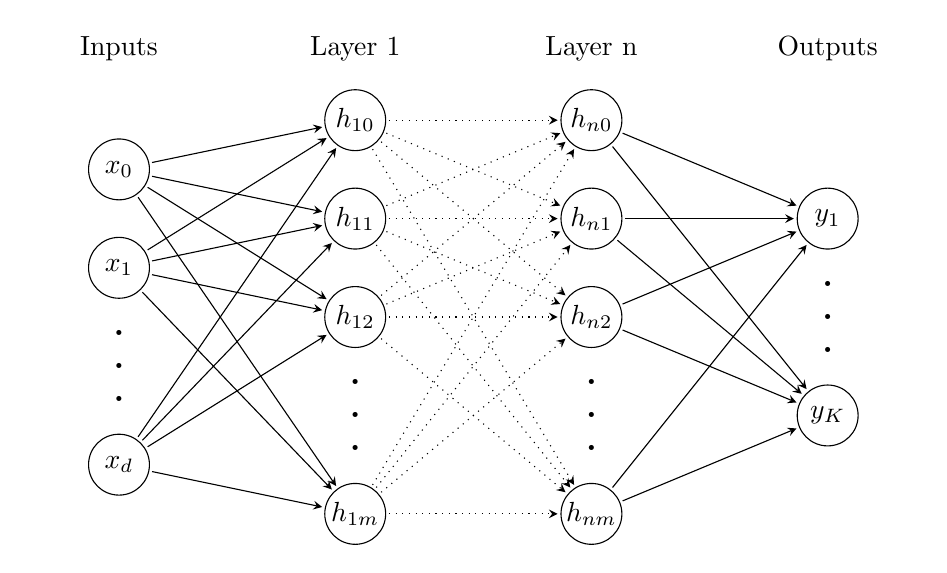
\begin{tikzpicture}[x=1.5cm, y=1.25cm, >=stealth]
    
    \foreach \m/\l [count=\y] in {1,2,missing,3}
    \node [every neuron/.try, neuron \m/.try] (input-\m) at (0,2-\y) {};

    \foreach \m [count=\y] in {1,2,3,missing,4}
    \node [every neuron/.try, neuron \m/.try ] (hidden1-\m) at (2,2.5-\y) {};

    \foreach \m [count=\y] in {1,2,3,missing,4}
    \node [every neuron/.try, neuron \m/.try ] (hidden2-\m) at (4,2.5-\y) {};

    \foreach \m [count=\y] in {1,missing,2}
    \node [every neuron/.try, neuron \m/.try ] (output-\m) at (6,1.5-\y) {};

    \foreach \l [count=\i] in {0,1,d}
    \node at (input-\i.center) {$x_{\l}$};

    \foreach \l [count=\i] in {0,1,2,m}
    \node at (hidden1-\i.center) {$h_{1\l}$};

    \foreach \l [count=\i] in {0,1,2,m}
    \node at (hidden2-\i.center) {$h_{n\l}$};

    \foreach \l [count=\i] in {1,K}
    \node at (output-\i.center) {$y_\l$};

    \foreach \i in {1,...,3}
    \foreach \j in {1,...,4}
    \draw [->, shorten <=1pt, shorten >=1pt] (input-\i) -- (hidden1-\j);

    \foreach \i in {1,...,4}
    \foreach \j in {1,...,4}
    \draw [dotted, ->, shorten <=1pt, shorten >=1pt] (hidden1-\i) -- (hidden2-\j);

    \foreach \i in {1,...,4}
    \foreach \j in {1,...,2}
    \draw [->, shorten <=1pt, shorten >=1pt] (hidden2-\i) -- (output-\j);

    \foreach \l [count=\x from 0] in {Inputs, Layer 1, Layer n, Outputs}
    \node [align=center, above] at (\x*2,2) {\l};
  \end{tikzpicture}
  \caption[A depiction of a neural network.]{A more complex neural network
    containing an input layer of $d$ nodes corresponding to data of dimensionality
    $d$, $n$ hidden layers of $m$ hidden units each $h_{ij}$ (where $i$ indexes
    hidden layer and $j$ indexes a particular unit) and an output layer of $K$
    predictive units $y_k$.}
  \label{fig:nn}
\end{figure}
There are now a great deal of parameters that we have to keep track of. It
is therefore important to distinguish between adaptive parameters and the
parameters which we must pick by hand, known as hyper-parameters. A relationship
can be written between the number of hidden layers $n$, and the number of
hyper-parameters, as follows
\begin{equation}
\text{\# of hyper-parameters} = 2n + 1.
\label{eq:hyper}
\end{equation}
As previously stated there are simply $n$ lots of activation functions and $n$
hidden layers to determine a size for. Often it is sufficient to set all
activation functions to the same function, and in this work all hidden layers
share the same size for simplicity. The adaptive parameters are far more
numerous, and will be optimised by means of a training algorithm. In TensorFlow
the variable object is choice for implementing the adaptive parameters as
training algorithms in the software will update them by default. The adaptive
parameters are initialised randomly from a Gaussian distribution resulting in
poor predictive power to begin with. In order to improve this some figure of
merit, known as a loss function, must be used in order for the training
algorithm to measure quantitatively the performance of the NN. We also must
provide the algorithm with a dataset to train on, complete with a set of targets
or labels that, for the training set, reveal the correct classification for each
entry. Due to the this requirement, methods such as these are referred to as
supervised learning methods. A natural loss function one may use to describe the
error of the model given a current set of adaptive parameters is sum-of-squares
error
\begin{equation}
E(\vec{w}) = \frac{1}{2}\sum_{n=1}^{N}(y(\vec{x}_n, \vec{w}) - t_n)^2
\label{eq:sumofsquares}
\end{equation}
where $t_n$ are the targets for the given data entries $\vec{x}_n$.
Minimising this function with some algorithm does work in practice, however it
has been shown that, using
\begin{equation}
E(\vec{w}) = - \sum_{n=1}^{N} \Bigg (t_n \ln (y_n) + (1-t_n) \ln (1-y_n) \Bigg)
\label{eq:xentropy}
\end{equation}
known as cross-entropy, is faster and more generalised \cite{XEntropySimard}
(further discussion on generalisation in section \ref{sec:generalisation}). The
particular training algorithm that will be used to update parameters in this
report is known as adaptive moment estimation or ADAM \cite{ADAMOpt}. ADAM is a
variant of the gradient descent algorithm, which is widely used and has spawned
many other variants \cite{GDOverview}. The reasons for picking between ADAM and
vanilla gradient descent are given in chapter \ref{ch:netarch}.

\tikzset{%
  every neuron/.style={
    circle,
    minimum size=22pt,
    draw
  },
  neuron missing/.style={
    draw=none, 
    scale=3,
    text height=0.3cm,
    execute at end node=\color{black}\tiny{$\vdots$}
  },
}

\begin{figure}[hbtp]
  \centering
  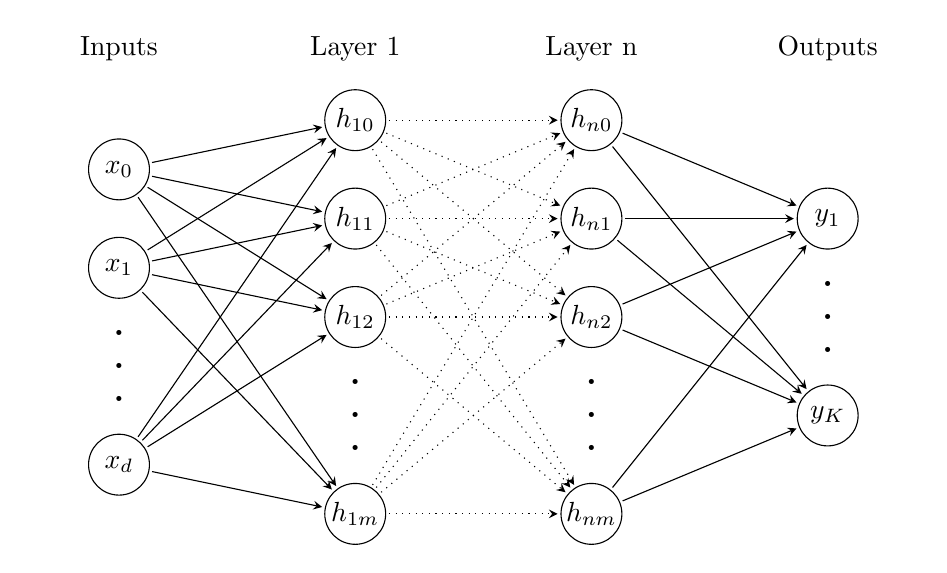
\begin{tikzpicture}[x=1.5cm, y=1.25cm, >=stealth]
    
    \foreach \m/\l [count=\y] in {1,2,missing,3}
    \node [every neuron/.try, neuron \m/.try] (input-\m) at (0,2-\y) {};

    \foreach \m [count=\y] in {1,2,3,missing,4}
    \node [every neuron/.try, neuron \m/.try ] (hidden1-\m) at (2,2.5-\y) {};

    \foreach \m [count=\y] in {1,2,3,missing,4}
    \node [every neuron/.try, neuron \m/.try ] (hidden2-\m) at (4,2.5-\y) {};

    \foreach \m [count=\y] in {1,missing,2}
    \node [every neuron/.try, neuron \m/.try ] (output-\m) at (6,1.5-\y) {};

    \foreach \l [count=\i] in {0,1,d}
    \node at (input-\i.center) {$x_{\l}$};

    \foreach \l [count=\i] in {0,1,2,m}
    \node at (hidden1-\i.center) {$h_{1\l}$};

    \foreach \l [count=\i] in {0,1,2,m}
    \node at (hidden2-\i.center) {$h_{n\l}$};

    \foreach \l [count=\i] in {1,K}
    \node at (output-\i.center) {$y_\l$};

    \foreach \i in {1,...,3}
    \foreach \j in {1,...,4}
    \draw [->, shorten <=1pt, shorten >=1pt] (input-\i) -- (hidden1-\j);

    \foreach \i in {1,...,4}
    \foreach \j in {1,...,4}
    \draw [dotted, ->, shorten <=1pt, shorten >=1pt] (hidden1-\i) -- (hidden2-\j);

    \foreach \i in {1,...,4}
    \foreach \j in {1,...,2}
    \draw [->, shorten <=1pt, shorten >=1pt] (hidden2-\i) -- (output-\j);

    \foreach \l [count=\x from 0] in {Inputs, Layer 1, Layer n, Outputs}
    \node [align=center, above] at (\x*2,2) {\l};
  \end{tikzpicture}
  \caption[A depiction of a neural network.]{A more complex neural network
    containing an input layer of $d$ nodes corresponding to data of dimensionality
    $d$, $n$ hidden layers of $m$ hidden units each $h_{ij}$ (where $i$ indexes
    hidden layer and $j$ indexes a particular unit) and an output layer of $K$
    predictive units $y_k$.}
  \label{fig:nn}
\end{figure}
\section{Parametrised Neural Networks}%
\label{sec:param-neural-nets}
Parametrised neural networks take extra inputs equal to the number of relevant
parameters, as seen in figure~\ref{fig:pnn}.
% UNUSED
% \begin{figure}[hbtp]
% \begin{center}
% \begin{tikzpicture}[x=1.5cm, y=1.25cm, >=stealth]

% \foreach \m/\l [count=\y] in {1,2,missing,3}
%   \node [every neuron/.try, neuron \m/.try] (input-\m) at (0,2-\y) {};

% \foreach \m [count=\y] in {1,2,3,missing,4}
%   \node [every neuron/.try, neuron \m/.try ] (hidden1-\m) at (2,2.5-\y) {};

% \foreach \m [count=\y] in {1,2,3,missing,4}
%   \node [every neuron/.try, neuron \m/.try ] (hidden2-\m) at (4,2.5-\y) {};

% \foreach \m [count=\y] in {1,missing,2}
%   \node [every neuron/.try, neuron \m/.try ] (output-\m) at (6,1.5-\y) {};

% \foreach \l [count=\i] in {0,1,d}
%   \node at (input-\i.center) {$x_{\l}$};

% \foreach \l [count=\i] in {0,1,2,m}
%   \node at (hidden1-\i.center) {$h_{1\l}$};

%   \foreach \l [count=\i] in {0,1,2,m}
%   \node at (hidden2-\i.center) {$h_{n\l}$};

% \foreach \l [count=\i] in {1,K}
%   \node at (output-\i.center) {$y_\l$};

% \foreach \i in {1,...,3}
%   \foreach \j in {1,...,4}
%     \draw [->, shorten <=1pt, shorten >=1pt] (input-\i) -- (hidden1-\j);

% \foreach \i in {1,...,4}
%   \foreach \j in {1,...,4}
%     \draw [dotted, ->, shorten <=1pt, shorten >=1pt] (hidden1-\i) -- (hidden2-\j);

% \foreach \i in {1,...,4}
%   \foreach \j in {1,...,2}
%     \draw [->, shorten <=1pt, shorten >=1pt] (hidden2-\i) -- (output-\j);

% \foreach \l [count=\x from 0] in {Inputs, Layer 1, Layer n, Outputs}
%   \node [align=center, above] at (\x*2,2) {\l};

% \end{tikzpicture}
% \caption{A more complex neural network containing an input layer of $d$ nodes corresponding to data of dimensionality $d$, $n$ hidden layers of $m$ hidden units each $h_{ij}$ (where $i$ indexes hidden layer and $j$ indexes a particular unit) and an output layer of $K$ predictive units $y_k$.}
% \label{fig:pnn}
% \end{center}
% \end{figure}


